% $Id: calculations-grooming.tex 515 2019-04-15 13:38:51Z gsoyez $
%
% This chapter contains the pQCD calculations for the grommed jet mass
%------------------------------------------------------------------------

\chapter{Calculations for the jet mass with grooming}\label{calculations-substructure-mass}

In this chapter we will revisit the calculations performed in Chapter~\ref{chap:calculations-jets} and extend them 
in order to describe jet mass distributions with grooming algorithms. 
%
In what follows, we are not going to present state-of-the art theoretical calculations, but instead we aim to keep the 
our discussion as simple as possible. Therefore, the theoretical accuracy of the calculations that we will present will be the minimum one which is required to capture the essential feature of the distributions. 
%
We will mostly concentrate of QCD jets, which present the most interesting and intricate features, while a discussion about jets originated to a boosted heavy particles will be presented in Sec.~\ref{sec:calc-groomed-mass-signal}.


%%========================================================================
\section{mMDT/ \SD mass}\label{sec:calc-groomed-mass}

The first calculation we perform is that of the invariant mass distribution of a jet after the mMDT / \SD algorithm
has been applied. As we have already mentioned, the \SD drop algorithm reduces to mMDT when the angular exponent
$\beta$ is set to zero. Therefore, in order to keep our notation light we are going to generically refer to the algorithm as \SD (SD) and it is understood that the $\beta=0$ case corresponds to mMDT.

In the next subsection, we do the calculation at leading order in the
strong coupling constant. This simple example will allow us to see the
large logarithms that appear and we will turn to their resummation in
the next subsection.

\subsection{LO calculation}\label{sec:calc-groomed-mass-LO}

\begin{figure}[t!]
  \centerline{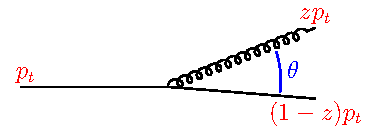
\includegraphics[width=0.45\textwidth]{figures/q2qg.pdf}}
  % 
  \caption{Diagram contributing to the leading-order mass
    distribution.}\label{fig:mmdt-mass-one-gluon}  
\end{figure}

At zeroth order in $\alpha_s$, the jet mass is always zero. To obtain
a non-trivial mass, we therefore need to consider a high-energy
parton, say a quark for definiteness, radiating an extra gluon, as
depicted in Fig.~\ref{fig:mmdt-mass-one-gluon}.
%
We want to focus on the boosted jet limit and highlight large
logarithms of $m/p_t$, with $p_t$ the transverse momentum of the
initial quark, which arise in the perturbative series expansion.
%
At the leading-logarithmic accuracy we are interested in, we can work
in the collinear approximation where the gluon emission angle $\theta$
is small.\footnote{Alternatively, we can assume a small jet radius $R$
  so that corrections beyond the collinear approximation are
  suppressed by powers of $R$. Note also that in the case of the mMDT
  jet mass, the SD condition actually gets rid of this
  contribution so that the collinear approximation remains valid at
  higher logarithmic accuracy.}
%
The gluon is set to carry a fraction $z$ of the quark momentum,
leaving a fraction $1-z$ for the recoiling quark after the emission.


When applying SD, the jet is split into two subjets, one
with the quark and one with the gluon which is tested for the
SD condition. Two situations can occur: (i) either the splitting
passes the SD condition, i.e. \ $z>\zcut (\theta/R)^\beta$ in
which case the quark-gluon system is retained by the SD procedure
and the (squared) jet mass is given by
\begin{equation}\label{eq:mmdt-qg-mass}
m^2 = z(1-z)\theta^2 p_t^2,
\end{equation}
or (ii) the condition is failed in which case only the harder of the quark
and the gluon is kept and the jet mass vanishes.
%
The mass distribution at LO is therefore given by
\begin{equation}\label{eq:mmdt-lo-full}
  \frac{m^2}{\sigma}\frac{d\sigma^{\text{(LO)}}}{dm^2}
  = \frac{\alpha_s}{2\pi} \int_0^{R^2}\frac{d\theta^2}{\theta^2}\int_0^1dz\,P_q(z)
  m^2\delta(m^2-z(1-z)\theta^2 p_t^2)\Theta\big(z>\zcut(\theta/R)^\beta\big),
\end{equation}
where $P_q(z)$ is the quark splitting function.

The mass constraint can be used to perform the integration over
$\theta$, and the constraint $\theta<R$ means we have to impose
$z(1-z)>\rho$ where we have introduced the dimensionless variable
\begin{equation}\label{eq:rho-definition}
  \rho = \frac{m^2}{p_t^2R^2}.
\end{equation}
Up to power corrections in $\rho$, i.e. in the groomed jet mass, we
can neglect the factor $1-z$ in this constraint.
%
We are therefore left with
\begin{equation}\label{eq:LOmmdtSD-zinteg}
  \frac{\rho}{\sigma}\frac{d\sigma^{\text{(LO)}}}{d\rho}
  = \frac{\alpha_s}{2\pi} \int_\rho^1dz\,P_q(z)
  \Theta\big(z^{2+\beta/2}>\zcut^{2/(2+\beta)}\rho^{\beta/(2+\beta)}\big).
\end{equation}
In the remaining integration over $z$, the SD constraint is only
relevant for $\rho<\zcut$ and we get 
%
\begin{equation} \label{eq:sigma-SD-LO}
  \frac{\rho}{\sigma}\frac{d\sigma^{\text{(LO)}}_\text{SD}}{d\rho} =
  \begin{cases}
   \frac{\alpha_sC_F}{\pi}
    \bigg[\log\Big(\frac{1}{\rho}\Big)-\frac{3}{4}\bigg],
  \quad \text{if} \quad \rho>\zcut,  \\
    \frac{\alpha_sC_F}{\pi}
    \bigg[\frac{\beta}{2+\beta}\log\Big(\frac{1}{\rho}\Big)+\frac{2}{2+\beta}\log\Big(\frac{1}{\zcut}\Big)-\frac{3}{4}\bigg],
  \quad \text{if} \quad \rho<\zcut,
  \end{cases}
\end{equation}
again up to power corrections in $\rho$.\footnote{Technically, for
  mMDT, this result is valid up to power corrections in $\zcut$. These
  corrections can be included and
  resummed~\cite{Dasgupta:2013ihk,Marzani:2017mva} but we will assume
  small $\zcut$ here and neglect them.}
%
The above result exhibits two different regimes: when the jet mass is
not very small $\rho>\zcut$, SD is inactive and one recovers the
plain, i.e.\ ungroomed jet-mass distribution discussed in Chapter~\ref{chap:calculations-jets}. However, when the mass becomes
smaller, $\rho<\zcut$, SD becomes active, as manifested here
under the form of a larger cut on the $z$ integration in Eq.~(\ref{eq:LOmmdtSD-zinteg}).

As mentioned in Chapter~\ref{chap:calculations-jets}, it is usual to
work with the cumulative distribution. At ${\cal O}(\alpha_s)$, we
find
%
\begin{align}
  \Sigma_{\text{SD}}^{\text{(LO)}}(\rho)
  & = \frac{1}{\sigma_0}\int_0^\rho d\rho' \frac{d\sigma}{d\rho'}
  = 1-\frac{1}{\sigma_0}\int_\rho^1 d\rho' \frac{d\sigma}{d\rho'}  \label{eq:mmdtsd-lo-cumul} \\
  & =
  \begin{cases}
     1- \frac{\alpha_sC_F}{\pi}
    \Big[\frac{1}{2}\log^2\big(\frac{1}{\rho}\big)-\frac{3}{4}\log\big(\frac{1}{\rho}\big)\Big], &
  \text{if} \quad \rho>\zcut, \\
    1- \frac{\alpha_sC_F}{\pi}
    \Big[\frac{1}{2}\log^2\big(\frac{1}{\rho}\big)-\frac{1}{2+\beta}\log^2\big(\frac{\zcut}{\rho}\big)-\frac{3}{4}\log\big(\frac{1}{\rho}\big)\Big], &
  \text{if} \quad \rho<\zcut.
  \end{cases}\nonumber
\end{align}

In going from the first to the second equality, one could either argue that
the probability is conserved (\ie the mass is either larger or
smaller than $\rho$), or realise that $\frac{d\sigma}{d\rho'}$ also
has a virtual contribution at $\rho'=0$ which, up to subleading power
corrections, can be written as
\[
  \left. \frac{d\sigma^{\text{(LO)}}}{d\rho'}\right|_{\text{virt.}}
   = -\bigg(\int_0^1 d\rho \frac{d\sigma}{d\rho}\bigg)\,\delta(\rho').
\]
More importantly, the results above clearly show that a gluon emission
comes with large logarithms of the jet mass on top the expected power
of $\alpha_s$. When the jet mass becomes sufficiently small, this is
no longer a small quantity and one needs to resum gluon emissions to
all orders. We do that in the next section.
%
There are however a few interesting points we can already highlight now.
%
For example, we see that the dominant logarithms in $\Sigma(\rho)$ are
double logarithms of the jet mass. These are associated with the
emission of a gluon which is both soft and collinear. The subleading
single-logarithmic contribution comes here from a hard and collinear
gluon emission.
%
Then, one expects the SD condition to be less effective as
$\beta$ increases. This is indeed what one sees here since one tends
to the plain jet mass distribution in the limit
$\beta\to\infty$. Conversely, for $\beta= 0$, the double logarithm of
the jet mass disappears --- going back to
Eq.~\eqref{eq:LOmmdtSD-zinteg} the $z$ integration is cut at $\zcut$
for $\beta=0$, meaning that the soft emissions only produce a
logarithm of $\zcut$ instead of a combination of $\log(\zcut)$ and
$\log(\rho)$ for the generic case --- leaving a single-logarithmic
dominant term, which is purely collinear.  

We conclude this section with a discussion about soft emissions at
large angles. These have not been included in the calculation above
where we have worked in the collinear, small $R$,
approximation. However, as seen in
Chapter~\ref{chap:calculations-jets} (see \eg
Eq.~(\ref{eq:sigma-1-loop-cntd})), soft emissions at finite angles can
also give single-logarithmic contributions.
%
This will no longer be the case in the region where SD is
active. To see this, imagine that we have a soft emission passing the
SD condition and dominating the jet mass. This implies
$\rho=z(\theta/R)^2$ and $z>\zcut (\theta/R)^\beta$, from which one
easily deduces $\theta<R (\rho/\zcut)^{1/(2+\beta)}$. A contribution
at a finite angle (\ie not enhanced by a collinear $d\theta/\theta$)
would therefore be suppressed by a power of $\rho$.
%
Similarly, one can show that non-global logarithms are also suppressed
by SD.
%
This is a fundamental analytic property of SD, namely that it
suppresses soft-and-large-angle gluon emissions so that observables can
(usually) be computed in the collinear limit. We will come back to
that point in the next section.

%%========================================================================
\subsection{Resummation of the mMDT/\SD mass distribution}\label{sec:calc-groomed-mass-LL}


We now move to the all-order resummation of the logarithms of the SD
jet mass distribution. We target a modified leading-logarithmic
accuracy, \ie include the leading double-logarithmic terms as well as
the hard-collinear single-logarithmic contributions.

In an all-order calculation, one has two types of contributions to
consider. First, real emissions which fail the SD condition will be
groomed away by the SD procedure~\footnote{Strictly speaking, since SD
  stops the first time the condition is passed, this is only true for
  gluons at angles larger than the first emission passing the SD
  condition. However, such gluons cannot dominate the jet mass and so
  can be neglected. It is worth noting that for more complicated
  quantities, like jet shapes computed on a SD jet, this effect would
  have to be taken into account.}  and will therefore not contribute
to the jet mass. They will therefore cancel explicitly against the
corresponding virtual corrections.
%
We are therefore left with the case of the real gluons which pass the
SD condition and the associated virtual emissions. These gluons
will contribute to the jet mass.
%
The situation here is therefore exactly as the one discussed in
Sec.~\ref{sec:jet-mass-res} for the case of the plain jet mass but
now restricted to the gluons passing the SD condition.

At the end of the day, this means that, if we want to compute the
cumulative distribution $\Sigma_{\text{SD}}(\rho)$, we have to
veto all real emissions that, while passing the SD condition, would give a ``mass'' larger than $\rho$.
Real emissions outside the SD
region and emissions at smaller mass do not contribute to the jet
mass~\footnote{At full single-logarithmic accuracy, one would also get
  a contribution with multiple emissions contributing to the jet mass,
  These emission would again have to pass the SD condition and
  their resummation goes exactly as for the plain jet, yielding a
  factor $\exp(-R')/\Gamma(1+R')$ with $R'$ the derivative of the
  SD radiator given below.} and cancel against virtual
corrections. We are therefore left with a ``standard'' Sudakov-type
factor
\begin{equation}\label{eq:mMDTSD-ll}
 \Sigma_{\text{SD}}(\rho) = \exp\big[-R_{\text{SD}}(\rho)\big],
\end{equation}
with (measuring the angles in units of the jet radius $R$ for
convenience and $i=q,g$)
\begin{equation}\label{eq:mMDTSD-radiator}
 R_{\text{SD}}(\rho) = \int_0^1
 \frac{d\theta^2}{\theta^2}\,dz\,P_i(z) \frac{\alpha_s(z\theta p_tR)}{2\pi}
 \Theta(z\theta^2>\rho) \Theta(z>\zcut \theta^\beta).
\end{equation}
In a fixed-coupling approximation, $R_{\text{SD}}$ is the same as
the one-gluon emission result, Eq.~\eqref{eq:mmdtsd-lo-cumul}. Including
running-coupling corrections is straightforward. We choose the hard scale to be $p_t R$ and we write
\begin{equation}
\alpha_s(z\theta p_tR) = \frac{\alpha_s (p_tR)}{1+2\alpha_s\beta_0\log(z\theta)},
\end{equation}
and we perform the integration keeping only the leading double-logarithmic contributions from
soft-and-collinear emissions as well as hard-collinear branchings. For $\rho<\zcut$, we obtain
\begin{align}\label{eq:mMDTSD-radiator-modll}
  R_{\text{SD}}^{\text{(LL)}}(\rho)
    & = \frac{C_i}{2\pi\alpha_s\beta_0^2}
      \bigg[\frac{2+\beta}{1+\beta}W\Big(1-\frac{\lambda_c+(1+\beta)\lambda_\rho}{2+\beta}\Big)
      -\frac{W(1-\lambda_c)}{1+\beta}-2W\Big(1-\frac{\lambda_\rho}{2}\Big)\nonumber\\
    & \phantom{=\frac{C_i}{2\pi\alpha_s\beta_0^2} \quad}
      -2\alpha_s\beta_0B_i\log\Big(1-\frac{\lambda_\rho}{2}\Big)\bigg],
\end{align}
with
\[
  \lambda_\rho = 2\alpha_s\beta_0\log(1/\rho),\qquad
  \lambda_c = 2\alpha_s\beta_0\log(1/\zcut),\qquad
  \text{and}\quad
  W(x)=x\log(x).
\]
%
The first line in Eq.~(\ref{eq:mMDTSD-radiator-modll}) corresponds to
the double logarithms, while the second line comes from hard-collinear
splittings.
%
This expression covers both the case of quark- and gluon-initiated
jets, with the only difference between the two are the overall colour
factor ($C_i=C_F$ for quarks and $C_i=C_A$ for gluons) and the
contribution from hard-collinear splittings ($B_i=B_q$ or $B_i=B_g$,
see Appendix~\ref{chap:app-analytic-details}).
%
As before, we recover the plain-jet case in the limit
$\beta\to\infty$, while the distribution becomes single-logarithmic
for the mMDT case, i.e.\ $\beta=0$.
%
Note that it might be convenient to reabsorb the contribution
from hard-collinear splittings, the last term
of Eq.~(\ref{eq:mMDTSD-radiator-modll}), directly into the
double-logarithmic contribution. This gives an expression equivalent
to Eq.~(\ref{eq:mMDTSD-radiator-modll}) up to NNLL corrections:
\begin{align}\label{eq:mMDTSD-radiator-modll-altB}
  R_{\text{SD}}^{\text{(LL)}}(\rho)
    & = \frac{C_i}{2\pi\alpha_s\beta_0^2}
      \bigg[\frac{2+\beta}{1+\beta}W\Big(1-\frac{\lambda_c+(1+\beta)\lambda_\rho}{2+\beta}\Big)
      -\frac{W(1-\lambda_c)}{1+\beta}-2W\Big(1-\frac{\lambda_\rho+\lambda_B}{2}\Big)\nonumber\\
    & \phantom{=\frac{C_i}{2\pi\alpha_s\beta_0^2} \quad}
      +W(1-\lambda_B)\bigg],
\end{align}
with $\lambda_B=-2\alpha_s\beta_0B_i$. 
%
The pros and cons of this alternative treatment of the $B$ term are
further discussed in Appendix~\ref{chap:app-analytic-details}.
%
More generally, the $B$ terms can systematically be inserted in the LL
contributions by replacing the $z<1$ kinematic boundary by
$z<\exp(B_i)$.
%
This is the approach we have adopted for all the plots obtained from
analytic calculations in this chapter.


\begin{figure}[t!]
    \centering
  \subfloat[]{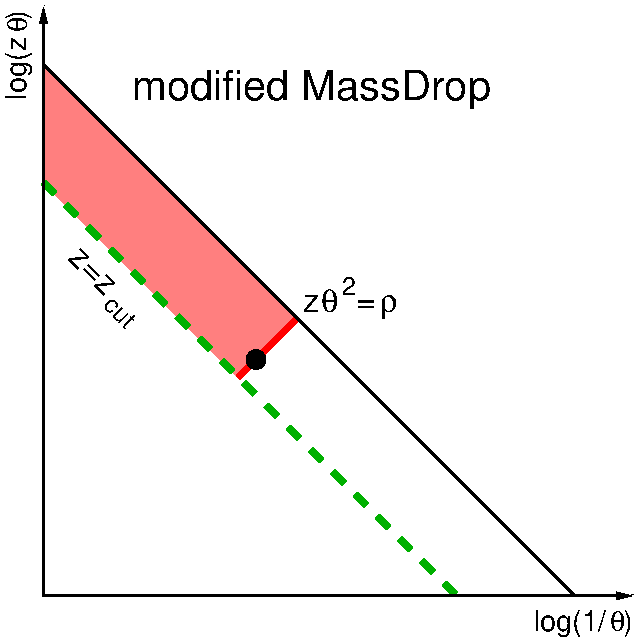
\includegraphics[width=0.45\textwidth]{figures/Lund-mMDT.pdf}%
    \label{fig:lund-mmdt}}%
  \qquad
  \subfloat[]{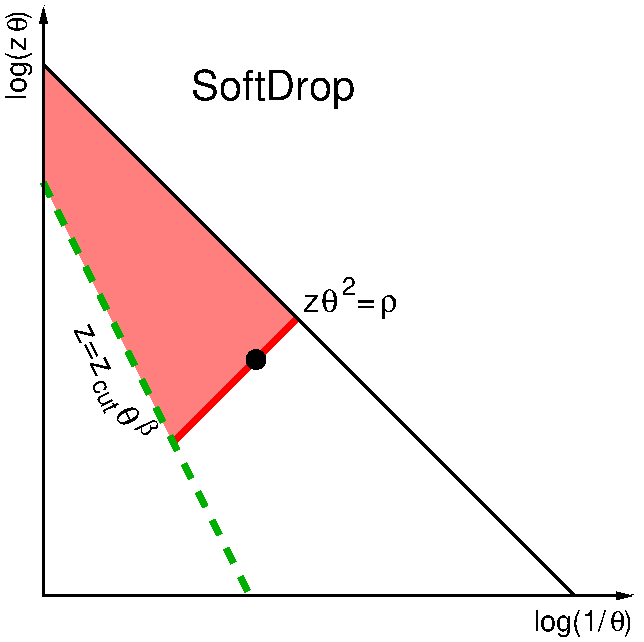
\includegraphics[width=0.45\textwidth]{figures/Lund-SD.pdf}%
    \label{fig:lund-sd}}%
  \caption{Lund diagrams for the groomed jet mass distribution at LL
    for mMDT (left) and generic SD (right). The solid green line
    represents the edge of the SD region, corresponding to the
    condition $z=\zcut\theta^\beta$. The solid red line corresponds to
    emissions yielding the requested jet mass, \ie satisfying
    $z\theta^2=\rho$. The shaded red area is the vetoed area
    associated with the Sudakov suppression.}\label{fig:lund-sd-mmdt}
\end{figure}

The above results can easily be represented using Lund diagrams
(cf.~\ref{sec:jet-mass-res}). This is done in
Fig.~\ref{fig:lund-sd-mmdt}. compared to the plain jet mass, only the
emissions above the SD condition have to be vetoed.
%
This corresponds to the shaded red region on the plot, therefore
corresponding to the radiator $R_{\text{SD}}$.
%
Similarly, its derivative with respect to $\log(1/\rho)$, $R'_{\text{SD}}$,
is the weight associated with having an emission passing the SD
condition and satisfying $z\theta^2=\rho$, and is represented by the
solid red line in Fig.~\ref{fig:lund-sd-mmdt}.
%
From both the analytic results and the simple Lund diagrams, one
clearly sees that the smaller $\beta$, the more aggressively one
grooms soft-and-large-angle emissions. Furthermore, when $\beta$ decreases,
both $R_{\text{SD}}$ and $R'_{\text{SD}}$ decrease.


%%========================================================================
\section{Other examples: trimming and pruning}\label{sec:calc-groomed-mass-others}

Amongst the taggers and groomers introduced in Chapter~\ref{tools},
the modified Mass-Drop Tagger and Soft~Drop are the ones with the
simpler analytic structure.
%
It is however possible to obtain results for other groomers/taggers as
well. In this section we give a brief overview of the mass
distribution one would obtain after applying trimming or pruning, as
initially calculated in Ref.~\cite{Dasgupta:2013ihk}.
%
We refer to Sec.~\ref{sec:tools-prong-finders-groomers} for a
description of the substructure tools.

\subsection{Trimming}

\paragraph{Leading-order result.} As above, we start with
${\cal O}(\alpha_s)$ calculation. Therefore, we consider a single soft
and collinear gluon emission in the jet, emitted from a high-energy
quark at an angle $\theta$ and carrying a fraction $z$ of the leading
parton's momentum.
%
For the jet mass to be non-zero, the emission needs to be kept in the
trimmed jet. 
%
If the emission is clustered in the same subjet as the leading parton,
it will automatically be kept; otherwise, if it is in its own subjet,
it will only be kept if it carries a fraction of the total jet $p_t$
larger than $f_\text{trim}$. After adding together real and virtual
contribution. the LO contribution to the cumulative distribution
is:\footnote{For brevity, the notation $\Theta(a\text{ or }b)$ is one
  if either $a$ or $b$ is satisfied and 0 is none of $a$ and $b$ are
  satisfied. It can be rewritten as
  $\Theta(a\text{ or
  }b)=\Theta(a)+(1-\Theta(a))\Theta(b)=\Theta(b)+(1-\Theta(b))\Theta(a)$.}
\begin{equation}\label{eq:trim-lo-full}
  \Sigma^{\text{(LO)}}_{\text{trim}}(\rho)
  = 1-\frac{\alpha_s}{2\pi} \int_0^1\frac{d\theta^2}{\theta^2}\int_0^1dz\,P_q(z)
  \,\Theta(z\theta^2>\rho)\,\Theta\big(z>\ftrim\text{ or }\theta<\rtrim\big),
\end{equation}
where we have introduced $\rtrim=\Rtrim/R$.
We note that the above expression  differs from the mMDT/SD case only by the tagger/groomer condition.
%
Therefore, if we are only interested in terms enhanced by logarithms of $\rho$,
$\ftrim$ or $\rtrim$, we can easily follow the same approach as in
Sec.~\ref{sec:calc-groomed-mass-LO} and get
%
\begin{align} \label{eq:trim-LO-result-cumulative}
 \Sigma_{\text{trim}}^{\text{(LO)}}(\rho)
  = 1- \frac{\alpha_sC_F}{\pi}
  &\bigg[\frac{1}{2}\log^2\Big(\frac{1}{\rho}\Big)-\frac{1}{2}\log^2\Big(\frac{\ftrim}{\rho}\Big)\Theta(\rho<\ftrim)\\
  &+\frac{1}{2}\log^2\Big(\frac{\ftrim\rtrim^2}{\rho}\Big)\Theta(\rho<\ftrim\rtrim^2)-\frac{3}{4}\log\Big(\frac{1}{\rho}\Big)\bigg],\nonumber
\end{align}
This results is very similar to what was obtained for the mMDT, i.e.\
Eq.~(\ref{eq:mmdtsd-lo-cumul}) with $\beta=0$, with one striking
difference: there is an additional transition point at
$\rho=\ftrim\rtrim^2$.
%
For $\ftrim\rtrim^2<\rho<\ftrim$, the distribution is
single-logarithmic and is the same as what one gets for $\rho<\zcut$
in the mMDT case with the replacement $\zcut\to \ftrim$. However, at lower
$\rho$, one has an extra contribution,
$\frac{1}{2}\log^2(\ftrim\rtrim^2/\rho)$, corresponding to a typical
plain-jet double-logarithmic contribution (albeit for a jet of
smaller radius).

For completeness, we also give the results for the differential mass
distribution at leading order, which reads
\begin{equation}  \label{eq:sigma-trimming-lo}
\frac{\rho}{\sigma} \frac{d\sigma^{\text{(LO)}}_\text{trim}}{d\rho}=
\begin{cases}
   \frac{\alpha_sC_F}{\pi}
    \Big[\log\big(\frac{1}{\rho}\big)-\frac{3}{4}\Big] \;
  &\text{if } \rho\ge\ftrim,\\
    \frac{\alpha_sC_F}{\pi}
    \Big[\log\big(\frac{1}{\ftrim}\big)-\frac{3}{4}\Big] \;
  &\text{if } \ftrim\rtrim^2\le\rho<\ftrim \\
   \frac{\alpha_sC_F}{\pi}
    \Big[\log\big(\frac{\rtrim^2}{\rho}\big)-\frac{3}{4}\Big] \;
  &\text{if } \rho<\ftrim\rtrim^2.
  \end{cases}
\end{equation}

\begin{figure}[t!]
  \centering
  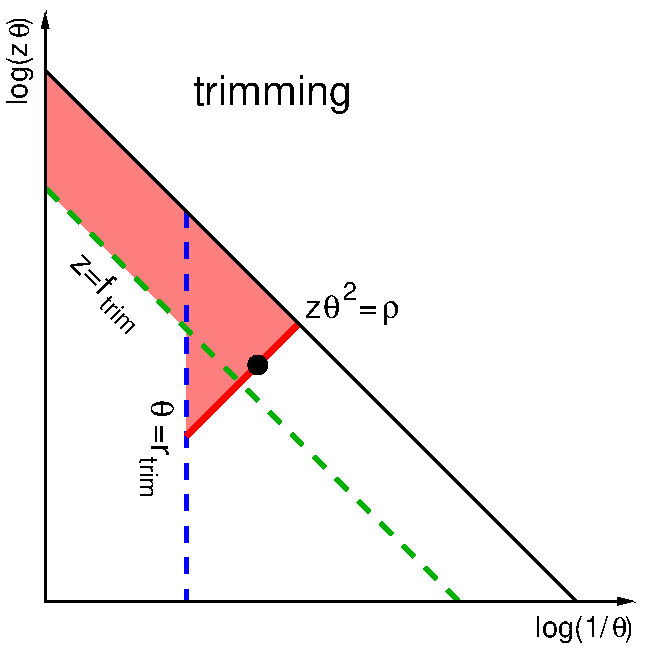
\includegraphics[width=0.45\textwidth]{figures/Lund-trim.pdf}%
  \caption{Lund diagrams for the trimmed jet mass distribution at LL
    for mMDT (left) and generic SD (right). The solid green and blue
    lines represents the edge of the trimming region, respectively
    representing the $z=\ftrim$ and $\theta=\Rtrim$ conditions.
    %
    The solid red line corresponds to emissions yielding the requested
    jet mass, \ie satisfying $z\theta^2=\rho$. The shaded red area is
    the vetoed area associated with the Sudakov
    suppression.}\label{fig:lund-trim}
\end{figure}
  

\paragraph{All-order resummation.} As for the \SD case, it is
relatively easy to show that the all-order resummed result is simply
the exponential of the one-gluon emission result (including
running-coupling corrections which we shall not explicitly calculate
here). We therefore get
\begin{equation}\label{eq:trim-ll}
 \Sigma_{\text{trim}}^{\text{(LL)}}(\rho) = \exp\big[-R_{\text{trim}}(\rho)\big],
\end{equation}
with, up to running-coupling corrections, 
\[
 R_{\text{trim}}(\rho) = 1-\Sigma_{\text{trim}}^{\text{(LO)}}(\rho).
\]
It is also informative to look at the corresponding Lund diagram,
plotted in Fig.~\ref{fig:lund-trim}. Compared to
Fig.~\ref{fig:lund-mmdt}, we explicitly see the emergence of a
transition point at $\rho=\ftrim\Rtrim^2$ and a double-logarithmic
behaviour in $\rho$ at smaller masses. This is associated with the
trimming radius $\Rtrim$ and the fact that emissions at angles smaller
than $\Rtrim$ will be kept in the groomed jet regardless of their
momentum fraction. This was different in the mMDT case where these emissions would still be
subject to the mMDT $\zcut$ constraint.

Finally, we can argue that this extra transition point is pathological
and a strong motivation to prefer the mMDT and \SD over trimming. Indeed, this
transition point produces a kink in the mass spectrum (see also
Sec.~\ref{sec:calc-groomed-mass-mc} below), smeared by subleading
contributions. Finding a possible signal in this region, or using this
mass domain as a side-band for a signal in an adjacent mass window,
would then become much more complex, if not impossible.
%
Additionally, this region would also receive single-logarithmic
contributions from soft-and-large angle emissions and non-global
logarithms (albeit suppressed by $\Rtrim^2$) which were absent in the
\SD case. 

Thus, all these factors render the calculation of the trimmed mass spectra of the same degree of complexity as the plain jet mass, if not worse because of the presence of the transition points. On the other hand, the analytic structure we have found for \SD was remarkable simpler and therefore amenable for precision calculations.

\subsection{Pruning}

In this section, we show explicitly that the case of pruning is more
complex but can be simplified by introducing instead the
Y-pruning variant. Since the main issue of pruning does not appear
in a LO calculation, we will briefly discuss its origin at NLO,
without providing an explicit calculation.
%
For simplicity, we take $f_{\text{prune}}=\frac{1}{2}$, so that the
pruning radius is given by $\Rprune=m_{\text{jet}}/p_{t,\text{jet}}$
and we introduce $\rprune=\Rprune/R$.

\paragraph{Leading-order result.} For a single soft-and-collinear
emission of momentum fraction $z$ and emission angle $\theta$, the jet
mass is given by $z\theta^2$, meaning that the pruning radius will be
set to $R_{\text{prune}}=\sqrt{z}\theta$ which is always smaller than
$\theta$. The emission will therefore be kept in the pruned jet only
if $z>\zprune$. This give exactly the same result as for mMDT, with
$\zcut$ replaced by $\zprune$:
\begin{equation}\label{eq:prune-lo-full}
  \Sigma^{\text{(LO)}}_{\text{prune}}(\rho)
   = \left.\Sigma^{\text{(LO)}}_{\text{mMDT}}(\rho)\right|_{\zcut\to\zprune},
\end{equation}
where we recall that mMDT corresponds to \SD with angular exponent $\beta=0$.

\paragraph{Behaviour at higher orders.} The pruning behaviour becomes significantly more complicated beyond LO. Let us give an explicit example. At NLO, we should consider
situations where we have two real emissions, 1 and 2, with respective
momentum fractions $z_1$ and $z_2$ and emission angles $\theta_1$ and
$\theta_2$ with respect to the leading parton (one should as well include the
cases with one or two virtual emissions).
%
Without loss of generality, we can assume that $z_1\theta_1^2\gg
z_2\theta_2^2$, with the strong ordering sufficient to capture the
leading logarithms of the jet mass we are interested in.
%
Emission 1 therefore dominates the (plain) jet mass and sets the
pruning radius to $R_{\text{prune}}=\sqrt{z_1}\theta_1$.
%
The complication comes from the fact that emission 1 itself may be
groomed away by pruning, \ie have $z_1<\zprune$, in which case, the
jet mass will only be non-zero if emission 2 is kept by pruning and
this is ensured by the condition
\[
  \Theta(z_2>\zprune\text{ or }\theta_2^2<z_1\theta_1^2),
\]
which depends on $z_1$. As we will see below, this is not a
show-stopper to resum the pruned jet mass distribution to all orders
but we definitely depart from the simple Sudakov exponentiation seen
for \SD, Eq.~(\ref{eq:mMDTSD-ll}), and trimming,
Eq.~(\ref{eq:trim-ll}).
%

\begin{figure}[t!]
    \centering
  \subfloat[]{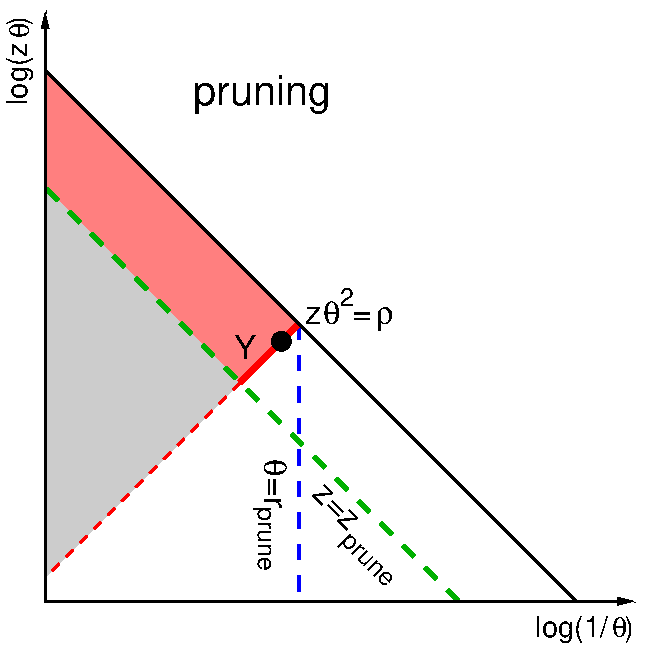
\includegraphics[width=0.32\textwidth]{figures/Lund-prune-case1.pdf}%
    \label{fig:lund-pruning-1}}\hfill%
  \subfloat[]{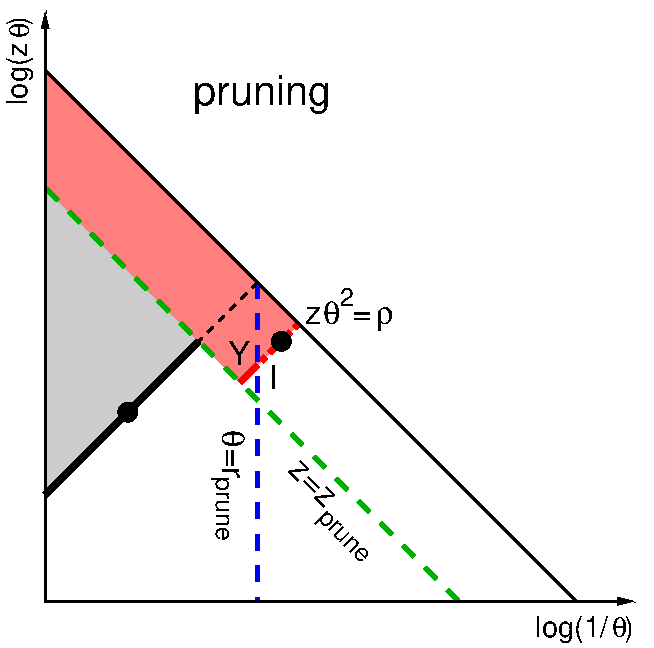
\includegraphics[width=0.32\textwidth]{figures/Lund-prune-case2a.pdf}%
    \label{fig:lund-pruning-2a}}\hfill%
  \subfloat[]{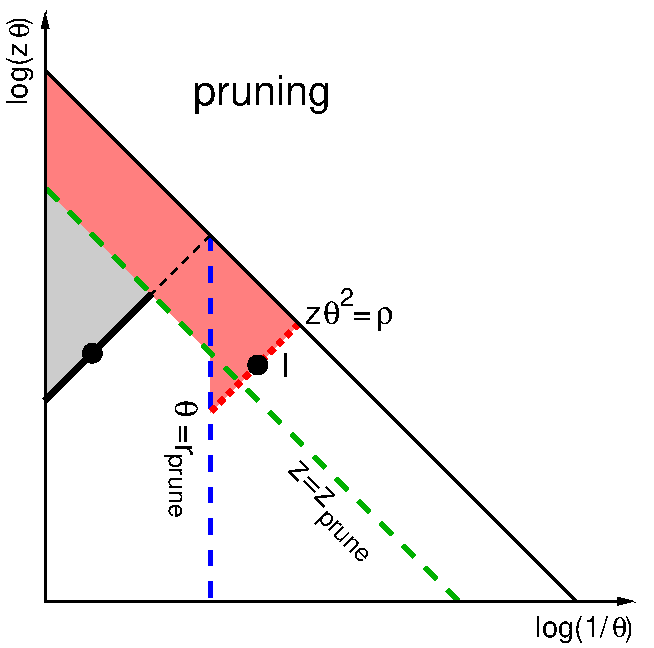
\includegraphics[width=0.32\textwidth]{figures/Lund-prune-case2b.pdf}%
    \label{fig:lund-pruning-2b}}%
  \caption{Lund diagrams for the groomed jet mass distribution at LL
    with pruning in three different kinematic configurations. In
    case~(a), the emission that dominates the plain jet mass (and
    hence sets the pruning radius) also has $z>\zprune$.
    % 
    In cases~(b) and~(c), the emission that dominates the plain mass
    and sets the pruning radius has $z<\zprune$ and does not pass the
    pruning condition.
    % 
    Another emission at lower mass dominates the pruned jet mass. This
    emission can either be constrained by the condition $z>\zprune$,
    case~(b), or by the condition $\theta>r_\text{prune}$, case~(c).
    %
    For each of the three cases, we indicate the contributions to Y-
    and I-pruning.}\label{fig:lund-pruning}
\end{figure}

\paragraph{All-order resummation.} 
%
To construct the all-order result, it is easier to consider the
differential jet mass distribution. Let us then denote by ``in'' the
emission that dominates the pruned jet, carrying a fraction $z_\text{in}$ of
the jet $p_t$ and emitted at an angle $\theta_\text{in}$, such that
$\rho=z_\text{in}\theta_\text{in}^2$.


The pruning radius in units of the original jet radius is given by
$\rprune^2=R_{\text{prune}}^2/R^2=m_{\text{jet}}^2/(p_{t,\text{jet}}R)^2$ which is set by the
emission dominating the plain jet mass.
%
We thus need to consider two cases: (i) there are no emissions in the
plain jet with $z\theta^2>z_\text{in}\theta_\text{in}^2$, (ii) there
is at least an emission in the plain jet with
$z\theta^2>z_\text{in}\theta_\text{in}^2$, and we call emission
``out'' the one with the largest $z\theta^2$, introducing
$\rho_\text{out}=z_\text{out}\theta_\text{out}^2$.
%
The corresponding Lund diagram is shown in
Fig.~\ref{fig:lund-pruning-1}.
%
In the first case, the pruning radius is set by emission one,
$r_{\text{prune}}^2=\rho<\theta_\text{in}^2$. To be in the pruned jet,
the ``in'' emission should therefore satisfy $z_\text{in}>\zprune$. We
get an associated Sudakov suppression $\exp(-R_\text{plain}(\rho))$
since we must veto emissions at larger mass than $\rho$ both in the
pruned jet and in the plain jet.
%
In the second case, the pruning radius is set by the ``out'' emission,
\ie $r_{\text{prune}}^2=\rho_\text{out}>\rho$. For
$\rho>\zprune\rho_{\text{out}}$, the pruning condition is then
$z_\text{in}>\zprune$ (shown in Fig.~\ref{fig:lund-pruning-2a}), while
for $\rho<\zprune\rho_{\text{out}}$ it becomes
$z_\text{in}>\rprune=\rho_\text{out}$
(Fig.~\ref{fig:lund-pruning-2b}).
%
The Sudakov receives two different contributions: one from inside the
pruning region, down to the scale $\rho$, represented by the red
shaded are in Fig.~\ref{fig:lund-pruning}, and one from outside the
pruning region, the grey area in Fig.~\ref{fig:lund-pruning}.
%
Note that since $\rho_\text{out}<\zprune$, the situation
$\rho<\zprune\rho_{\text{out}}$ only happens for $\rho<\zprune^2$,
yielding a transition point at $\rho=\zprune^2$.

For $\zprune^2<\rho<\zprune$, the sum over the two regions can be
written as
\begin{align}\label{eq:pruning-largerho-int}
  \frac{\rho}{\sigma}\frac{d\sigma_{\text{prune}}}{d\rho}
  &= \int_{\zprune}^1 dz_\text{in} P_i(z_\text{in})
    \frac{\alpha_s}{2\pi} e^{-R_\text{in}(\rho)}
    \bigg[
    e^{-R_\text{out}(\rho)}
    +\int_\rho^{\zprune}\frac{d\rho_\text{out}}{\rho_\text{out}}R'_\text{out}(\rho_\text{out})
    e^{-R_\text{out}(\rho_\text{out})}
    \bigg]\nonumber \\
  & = R'_\text{in}(\rho) e^{-R_\text{in}(\rho)}, \quad \text{with }\rho> \zprune^2,
\end{align}
where we have introduced the radiators
\begin{align}
  R_\text{in}(\rho) & = R_{\text{mMDT}}(\rho),\\
  R_\text{out}(\rho) & = R_{\text{plain}}(\rho)-R_{\text{mMDT}}(\rho),
\end{align}
where $R_{\text{mMDT}}$ is obtained by setting $\beta=0$ in Eq.~(\ref{eq:mMDTSD-radiator-modll}).
The radiators correspond respectively to the region kept (the shaded red area of
Fig.~\ref{fig:lund-pruning}) and rejected (the grey area of
Fig.~\ref{fig:lund-pruning}) by pruning. As long as the pruning
condition is only $z>\zprune$, as in the above case, the $R_\text{in}$
Sudakov is the same as the mMDT Sudakov,
Eqs.~(\ref{eq:mMDTSD-radiator}) and~(\ref{eq:mMDTSD-radiator-modll}).
%
The $R'_\text{out}$ factor in the first line of Eq.~(\ref{eq:pruning-largerho-int}) corresponds to the integral over the
momentum fraction of the emission outside the pruning region,
represented by the solid black line in Fig.~\ref{fig:lund-pruning}.
%
After integration, we find that the pruned jet mass distribution is
identical to the mMDT mass distribution for $\rho>\zprune^2$.

The situation for $\rho<\zprune^2$ is more involved as one now has to
include the situation from Fig.~\ref{fig:lund-pruning-2b} as well. In
that case, the $R_\text{in}$ Sudakov gets an additional contribution
and the lower bound of the $z_\text{in}$ integration extends down to
$\rprune$. We then write
%
\begin{align}\label{eq:pruning-smallrho-int}
  \frac{\rho}{\sigma}\frac{d\sigma_{\text{prune}}}{d\rho}
   = &\int_{\zprune}^1 dz_\text{in} P_i(z_\text{in})
    \frac{\alpha_s}{2\pi} e^{-R_\text{in}(\rho)}
    \bigg[
    e^{-R_\text{out}(\rho)}
    +\int_\rho^{\rho/\zprune}\frac{d\rho_\text{out}}{\rho_\text{out}}R'_\text{out}(\rho_\text{out})
    e^{-R_\text{out}(\rho_\text{out})}
    \bigg]\nonumber\\
  & + \int_{\rho/\zprune}^{\zprune}\frac{d\rho_\text{out}}{\rho_\text{out}}R'_\text{out}
    e^{-R_\text{out}(\rho)-R_\text{in}(\rho;\rho_\text{out})}
    \int_{\rho_\text{out}}^1 dz_\text{in} P_i(z_\text{in})
    \frac{\alpha_s}{2\pi} \nonumber \\
 =   & \, R'_\text{in}(\rho) e^{-R_\text{in}(\rho)-R_\text{out}(\frac{\rho}{\zprune})} 
  \nonumber \\
 &+ \int_{\rho/\zprune}^{\zprune}\frac{d\rho_\text{out}}{\rho_\text{out}}R'_\text{out}
    e^{-R_\text{out}(\rho)-R_\text{in}(\rho;\rho_\text{out})}
    \int_{\rho_\text{out}}^1 dz_\text{in} P_i(z_\text{in})
    \frac{\alpha_s}{2\pi}
\end{align}
with the new radiator
\begin{equation}
  R_\text{in}(\rho;\rho_\text{out})
  = \int_0^1 \frac{d\theta^2}{\theta^2}dz  P_i(z)\frac{\alpha_s}{2\pi}
  \Theta(z\theta^2>\rho) \Theta(z>{\text{min}}(\zprune,\rho_\text{out})),
\end{equation}
corresponding to the shaded red region of
Fig.~\ref{fig:lund-pruning-2b}.
%
Some simplifications and approximations can be done at fixed coupling
but the main message here is that at small $\rho$, $\rho<\zprune^2$,
the pruned mass distribution no longer involves a Sudakov which is the
simple exponentiation of the one-gluon-emission result. In that
region, one is left with an additional integration over the plain jet
mass $\rho_\text{out}$ which gives a Sudakov with double logarithms of
the pruned jet mass $\rho$.

\paragraph{Y-pruning and I-pruning.} The main complication of
pruning originates from the situation depicted in Fig.~\ref{fig:lund-pruning-2b},
where the pruning radius is set by an emission which is groomed away. 
and the pruned mass is dominated by an emission at an angle smaller
than the pruning radius. 
In this situation the prune radius is anomalously large because it is not set by hard splitting, as one would physically expect from pruning, especially when it is used as a two-prong tagger and the pruned jet is characterised by just one hard prong, hence the name I-pruning. 
Conversely, Y-pruning configurations are characterised by a hard $1\to 2$ splitting. 
It is therefore interesting to compute the jet mass for Y-pruning.

The situation of Fig.~\ref{fig:lund-pruning-2b} where the emission that
dominates the pruned jet mass always has $\theta<\rprune$ is of the
I-pruning type and does not contribute at all to Y-pruning.
%
This is already a great simplification since, for example, all the
expressions will now involve the simple $R_\text{in}(\rho)$ Sudakov
and no longer $R_\text{in}(\rho';\rho_\text{out})$.
%
Furthermore, for the cases where the emission setting the pruned mass
also sets the plain jet mass, Fig.~\ref{fig:lund-pruning-1}, we always
have $z_\text{in}>\zprune$ and
$\theta_\text{in}>\rprune=\sqrt{z_\text{in}}\theta_\text{in}$, meaning that
this situation is always of the Y-pruning type.

Unfortunately, there is a price to pay for the remaining contribution,
Fig.~\ref{fig:lund-pruning-2a} for which, as indicated on the figure,
one only gets a jet contributing to Y-pruning for smaller values of
$z_\text{in}$, namely for
$\zprune<z_\text{in}<\rho/\rho_\text{out}$.\footnote{This argument is
  not entirely true since even for $z_\text{in}>\rho/\rho_\text{out}$
  we could still have another emission with $z>\zprune$,
  $\theta>\rprune$ and $z\theta^2<\rho$. Such a contribution would
  only give terms proportional to $\alpha_s\log^2(\zprune)$ i.e.\ not
  enhanced by any logarithm of the jet mass. We therefore neglect
  these contributions here.}
%
Taking this into account, the Y-pruned jet mass distribution can
be written as  (assuming $\rho<\zprune$)
\begin{align}
  \frac{\rho}{\sigma}\frac{d\sigma}{d\rho}
   & = \int_{\zprune}^1 dz_\text{in} P_i(z_\text{in})
   \frac{\alpha_s}{2\pi} e^{-R_\text{plain}(\rho)}\\
   & + \int_\rho^{\text{min}(\zprune,\rho/\zprune)}\frac{d\rho_\text{out}}{\rho_\text{out}}R'_\text{out}(\rho_\text{out})
    e^{-R_\text{out}(\rho_\text{out})-R_\text{in}(\rho)}
     \int_{\zprune}^{\rho/\rho_\text{out}} dz_\text{in} P_i(z_\text{in}).\nonumber
\end{align}
Inverting the two integrations on the second line, one can perform
explicitly the integration over $\rho_\text{out}$ and keep only an
integration over $z_\text{in}$:
\begin{equation}\label{eq:Ypruning}
  \frac{\rho}{\sigma}\frac{d\sigma}{d\rho}
    =  \int_{\zprune}^1 dz_\text{in} P_i(z_\text{in})
   \frac{\alpha_s}{2\pi} e^{-R_\text{in}(\rho)-R_\text{out}({\text{min}}(\zprune,\rho/z_\text{in}))}.
 \end{equation}
 The Sudakov in the $z_\text{in}$ integrand has a few interesting
 properties. First, for $\rho/z_\text{in}>\zprune$, it involves
 $R_\text{out}(\zprune)=0$ and we recover a behaviour similar to what
 was seen for the mMDT. For $\rho/z_\text{in}<\zprune$, which is
 always the case for $\rho<\zprune^2$, $R_\text{out}$ then becomes
 double-logarithmic in $\rho$.

 
\subsection{Non-perturbative corrections in groomed distributions}\label{sec:groomed-mass-hadronisation}

In Sec.~\ref{sec:plain-mass-hadronisation} we have provided a rough
estimate of the value of the jet mass at which the distribution
becomes sensitive to non-perturbative physics.
%
It is instructive to study revisit that calculation and see how this non-perturbative transition point changes if grooming techniques are applied. 

We start by considering trimming. Assuming that we are in the
$\rho < \ftrim \rtrim^2$ region, the situation is analogous to the
plain jet mass and the mass $m$ at which one becomes sensitive to
non-perturbative effects is the same as
Eq.~(\ref{eq:mass-NP-estimate}) but with the jet radius substituted by
the trimming radius
\begin{equation}\label{eq:mass-NP-estimate-trimming}
m^2\simeq \frac{\muNP}{p_t \Rtrim} p_t^2 \Rtrim^2= \muNP p_t \Rtrim,
\end{equation}
where, compared to Eq.~(\ref{eq:mass-NP-estimate}), we have switched
to hadron-collider variables and used $p_t$ rather than $E_J$.
%
For pruning (both Y- and I-configuration), the non-perturbative
transition point is formally the same as the plain jet mass,
essentially because it is the latter that sets the pruning
radius. Note however, that the size of non-perturbative corrections
can differ with respect to the plain mass and one does expect pruning
to achieve a significant reduction.

For the \SD case we need a new calculation. We have to work out when
an emission of constant $\rho = z \theta^2$, and passing the \SD
condition, first crosses into the non-perturbative region
$ z \theta< \tilde{\mu}=\frac{\muNP}{p_tR}$.
%
This happens at the maximum allowed (rescaled) angle ($\theta=1$ for
the plain mass) which is determined by the \SD condition
$z=\zcut \theta^\beta$. We obtain
$\rho\simeq \tilde{\mu} \left(\tfrac{\tilde{\mu}}{\zcut}
\right)^\frac{1}{1+\beta}$, which implies
\begin{equation}\label{eq:non-perturative-mass-SD}
m^2\simeq \muNP^\frac{2 +\beta}{1+\beta} \zcut^\frac{-1}{1+\beta}(p_t R)^\frac{\beta}{1+\beta}.
\end{equation}
Compared to the plain jet mass case,
Eq.~(\ref{eq:mass-NP-estimate}), the (squared) mass at which
one becomes sensitive to non-perturbative effects is therefore smaller
by a factor $\big(\tfrac{\muNP}{\zcut p_tR}\big)^{\frac{1}{1+\beta}}$.
%
Once again, we note that the mMDT limit $\beta=0$ is particularly
intriguing as the $p_t$ dependence disappears from
Eq.~\eqref{eq:non-perturative-mass-SD}.


 
\subsection{Summary and generic overview}

\begin{table}
  \centering
  \begin{tabular}{r|cccccc}
    Groomer/  & transition & exponen- & largest & soft & non-global & non-pert\\
    tagger    &  points & -tiates &  logs & logs &  logs  & $m^2$ scale\\
    \hline
    Plain     & -                         & yes & $\alpha_s^nL^{2n}$ &  yes  & yes & $\muNP p_tR$\\
    mMDT      & $\zcut$                   & yes & $\alpha_s^nL^{n}$ & no  & no & $\muNP^2/\zcut$\\
    SoftDrop  & $\zcut$                   & yes & $\alpha_s^nL^{2n}$ & no  & no & $(\tfrac{\muNP^{2+\beta}(p_tR)^\beta}{\zcut}\big)^{\frac{1}{1+\beta}}$\\
    trimming  & $\ftrim$,$\ftrim\rtrim^2$ & yes & $\alpha_s^nL^{2n}$ & yes & yes & $\muNP p_t\Rtrim$\\
    pruning   & $\zprune$,$\zprune^2$     & no  & $\alpha_s^nL^{2n}$ & yes & yes & $\muNP p_tR$\\
    Y-pruning & $\zprune$                 & no  & $\alpha_s^nL^{2n-1}$
                                                & yes & yes & $\muNP p_tR$\\
    \hline
  \end{tabular}
  \caption{Summary of the basic analytic properties of taggers. Here,
    $L=\log(\rho)$. By soft logs we mean logarithmic contributions
    originating from soft emissions at finite angle. We note that \SD
    does retain soft/collinear contributions (hence the double
    logarithmic behaviour), while mMDT only keeps hard-collinear
    radiation. 
  }\label{tab:groomers-analytic-props}
\end{table}

To conclude this section on analytic calculations, we summarise the
basic analytic properties of the groomers/taggers in
Table~\ref{tab:groomers-analytic-props}.

A few key observations can be made.
\begin{itemize}
\item The modified MassDropTagger and SoftDrop groom soft radiations
  at all angular scales, \ie without stopping at a given subjet
  radius. This has the consequence that they are insensitive to soft
  gluon emissions at finite angles and have no non-global logarithms.
  %
\item Another consequence of the absence of a subjet radius for mMDT
  and SD is that they are free of transition points beyond the one at
  $\rho=\zcut$. This is also the case of Y-pruning.
  %
  Transition points can have subtle consequences in phenomenological
  applications and are therefore best avoided if possible.
  %
  Furthermore, as we shall see explicitly in comparisons to Monte
  Carlo simulation in Sec.~\ref{sec:calc-groomed-mass-ps} below,
  for heavily boosted bosons these transition points can be around the
  electroweak scale and therefore have delicate side-effects when used
  in tagging boosted electroweak bosons.
  %
\item the simple symmetry cut of the mMDT, independent on the emission
  angles, translates into a perturbative logarithmic series where
  there are no double logarithms and the leading contributions are
  single logarithms of the jet mass.
  %
  Although this translates into a smaller Sudakov suppression of the
  QCD background, this has the advantage of being theoretically
  simple. This, together with the fact that the mMDT strongly reduces
  the sensitivity to non-perturbative effects (see
  Sec.~\ref{sec:calc-groomed-mass-mc} below), is why it is a tool
  with a great potential for precision physics at the LHC.
  %
\item For many of the groomers we have studied, the resummed result
  has a simple structure where the one-gluon-emission expression
  simply exponentiates. The main exception to that is pruning which
  does not exponentiate. The situation is partially alleviated in the
  Y-pruning case.
\end{itemize}



%%========================================================================
\section{Comparison to Monte Carlo}\label{sec:calc-groomed-mass-mc}

Now that we have obtained resummed results it is instructive to
compare our findings to Monte Carlo simulations, which are ubiquitously used in phenomenology.
 We first do that at
leading order to explicitly test the appearance of logarithms of the
jet mass and check our control over the associated coefficients. We
then move to a comparison to parton-shower simulations. In
this case we will also discuss the impact of non-perturbative effects.

\subsection{Comparisons at leading order}\label{sec:calc-groomed-mass-mc-lo}

An simple test of the above substructure calculations is to verify
that they do reproduce the logarithmic behaviour of a
fixed-order calculation.
%
To this purpose, we can use the
Event2~\cite{Catani:1996jh,Catani:1996vz} generator.
 Although the program generates $e^+e^-$ collisions,
one can simulate quark jets of a given $p_t$ (at $y=\pi=0$) by
rotating the whole event so that the thrust axis (or, alternatively
the axis of the reference $q\bar q$ event generated by Event2) aligns
with the $x$ axis.
%
We then cluster the jets with the anti-$k_t$
algorithm~\cite{Cacciari:2008gp}\footnote{At leading order,
  ${\cal {O}}(\alpha_s)$, one could equivalently use any algorithm in
  the generalised-$k_t$ family.} with $R=1$ (cf.
Chapter~\ref{chap:jets-and-algs}).
%
We then apply any groomer to the resulting jets and measure the
groomed jet mass.
%
In practice, we have used mMDT with $\zcut=0.1$, \SD with
$\beta=2$ and $\zcut=0.1$ and trimming with $\ftrim=0.1$ and
$\Rtrim=0.2$.
%
In this section, we focus on the lowest non-trivial order of
perturbation theory, ${\cal{O}}(\alpha_s)$. since we need at least 2
partons in a jet if we want a non-zero mass, it is sufficient to
consider the real gluon emissions, \ie $e^+e^-\to q\bar
q g$ events.


\begin{figure}[t!]
  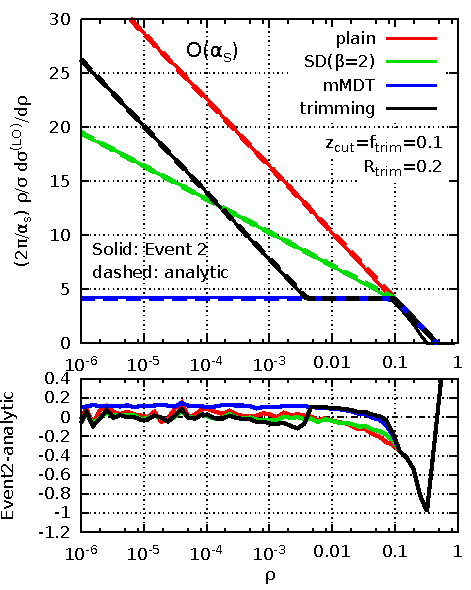
\includegraphics[width=0.5\textwidth]{figures/groomed-rho-event2.pdf}\hfill%
  \begin{minipage}[b]{0.42\textwidth}
    \caption{Comparison of the (normalised) mass distribution obtained
    at leading order, ${\cal{O}}(\alpha_s)$, between Event2 (solid
    lines) and our analytic expectations (dashed lines). The
    distribution is shown for both the plain jet (red) and a series of
    groomers: SoftDrop with $\beta=2$ (green), mMDT (blue) and
    trimming with $\Rtrim=0.2$ (black).
    %
    The lower panel shows the difference between Event2 and the
    associated analytic expectation.
  }\label{fig:groomers-event2}
    \vspace*{1.4cm}
  \end{minipage}\hspace*{0.3cm}
\end{figure}

Fig.~\ref{fig:groomers-event2} shows the mass distribution for a few
selected groomers, together with the analytic calculations from above,
expanded at order $\alpha_s$. For \SD, this is given by
Eq.~\eqref{eq:sigma-SD-LO}, while for trimming by
Eq.~\eqref{eq:sigma-trimming-lo}. At ${\cal {O}}(\alpha_s)$, pruning
and Y-pruning coincide with the mMDT and are therefore not showed.
%
The bottom panel of the plot shows the difference between the Event2
simulations and the analytic results.

All the features discussed in this chapter are clearly visible on this
plot: the transition points, at $\rho=\zcut$ for
SD and at $\rho=\ftrim$ and $\rho=\ftrim\rtrim^2$ for trimming,
are present in the exact Event2 simulation; the effect of grooming
is clearly visible at small $\rho$, with a reduction of the
cross-section; the reduced $\log(\rho)$ contribution with \SD and
the absence of the $\log(\rho)$ enhancement for mMDT; the equivalence of
trimming and mMDT in the intermediate $\rho$ region; and the
reappearance of the plain-mass-like $\log(\rho)$ contribution at small
$\rho$ for trimming.

Comparing the asymptotic behaviour at small mass to our
analytic calculation, we first see that the leading logarithmic
behaviour, \ie the $\log(\rho)$ contribution, is correctly
reproduced. This is visible on the bottom panel of
Fig.~\ref{fig:groomers-event2} where all curves tend to a constant at
small $\rho$.
%
Furthermore, for trimming and \SD, the analytic calculation also
captures the constant term --- $B_q=-\tfrac{3}{4}$ coming from
hard-collinear branchings --- and the difference between Event2 and the
analytic results vanishes at small $\rho$.
%
Although it is a bit delicate to see it on the figure, in the case of the
plain, ungroomed, jet, this difference is  only going to a non-zero
constant at small $\rho$, because our calculation is missing a finite
$R^2$ contribution coming from the emission of a soft gluon at a large
angle.
%
Finally, in the case of the mMDT, this difference is clearly different from 0 at small
$\rho$. This originates from the fact that our analytic calculation in
Sec.~\ref{sec:calc-groomed-mass} has assumed $\zcut\ll 1$. For a
finite value of $\zcut$, one has to keep the full $z$ dependence in
the splitting function which, at ${\cal{O}}(\alpha_s)$ means
\begin{equation}
  \frac{\rho}{\sigma}\frac{d\sigma_{\text{mMDT}}}{d\rho}
   =
   \frac{\alpha_sC_F}{2\pi}\int_{\zcut}^{1-\zcut}dz\,\frac{1+(1-z)^2}{z}
   = \frac{\alpha_sC_F}{\pi}\bigg[\log\Big(\frac{1-\zcut}{\zcut}\Big)-\frac{3}{4}(1-2\zcut)\bigg].
\end{equation}
Finite $\zcut$ effects are of then given by
$\tfrac{\alpha_sC_F}{\pi}\left[ \tfrac{3}{2}\zcut-\log(1-\zcut)\right]$. Pulling out
an $\tfrac{\alpha_s}{2\pi}$ factor as done in Event2 and in
Fig.~\ref{fig:groomers-event2}, this gives a difference around 0.12
for our choice of $\zcut=0.1$, which corresponds to what is observed
on the plot.
  
\subsection{Comparisons with parton shower}\label{sec:calc-groomed-mass-ps}

\begin{figure}[t!]
  \subfloat[]{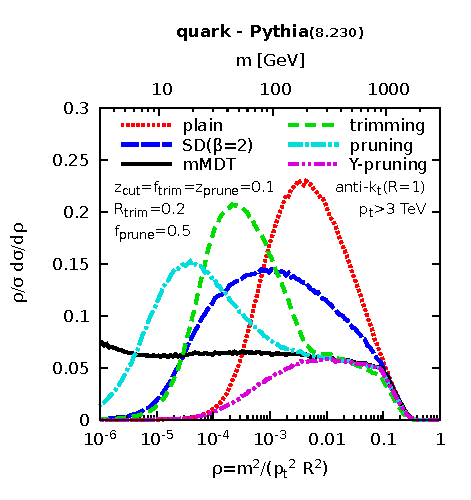
\includegraphics[width=0.48\textwidth,page=1]{figures/groomed-rho-pythia.pdf}\label{fig:groomers-pythia}}%
  \hfill%
  \subfloat[]{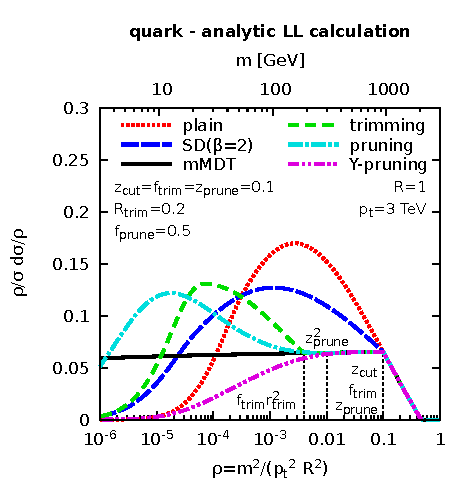
\includegraphics[width=0.48\textwidth,page=1]{figures/groomed-rho-analytic.pdf}\label{fig:groomers-analytic}}
  %
  \caption{Mass distribution obtained for the ungroomed jet (dotted,
    red) as well as with different groomers: SoftDrop($\beta=2$)
    (long-dashed, blue), mMDT (solid, black), trimming (short-dashed,
    green), pruning (dot-dashed, cyan) and Y-pruning (dot-dot-dashed,
    magenta). The left plot is the result of a Pythia parton-level
    simulation and the right plot is the analytic results discussed in
    this chapter.}\label{fig:groomers-pythia-v-analytic}
\end{figure}


\begin{figure}[t!]
  \subfloat[]{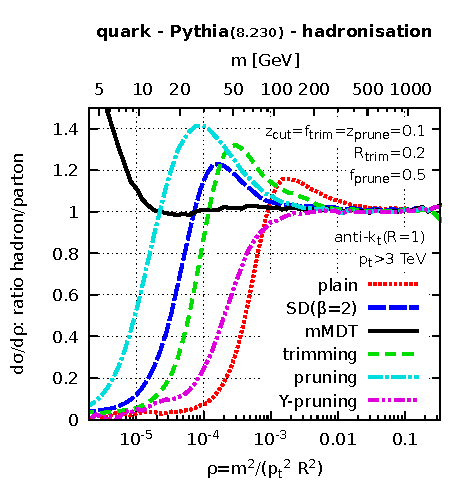
\includegraphics[width=0.48\textwidth,page=1]{figures/groomed-rho-pythia-np.pdf}\label{fig:groomer-pythia-hadr}}%
  \hfill%
  \subfloat[]{\includegraphics[width=0.48\textwidth,page=2]{figures/groomed-rho-pythia-np.pdf}\label{fig:groomer-pythia-ue}}
  %
  \caption{Non-perturbative effects on the groomed jet mass
    distribution. The lines are as in
    Fig.~\ref{fig:groomers-pythia-v-analytic}. All results are
    obtained from Pythia8 simulations. The left plot corresponds to
    hadronisation effects, \ie the ratio of hadron-level to
    parton-level distributions. The right plot shows the effects of the
    UE, \ie the ratio of the mass distribution with UE
    effects on and off.}\label{fig:groomers-pythia-npeffects}
\end{figure}

\paragraph{Setup.}
%
We now compare our all-order results, including running coupling, to a
full parton-shower simulation.
%
For this, we use the Pythia8~\cite{Sjostrand:2014zea} generator, in
its Monash13 tune~\cite{Skands:2014pea} at parton level. We generate
dijet events at $\sqrt{s}=13$~TeV, restricting the hard matrix element
to $qq\to qq$ processes.
%
Jets are reconstructed with the anti-$k_t$ algorithm, as implemented
in FastJet~\cite{Cacciari:2005hq,Cacciari:2011ma}, with $R=1$,
keeping only jets with $p_t>3$~TeV and $|y|<4$,
%
We study the same groomers as for the Event2 study, as well as pruning
and Y-pruning with $\zprune=0.1$ and $f_\text{prune}=0.5$.

\paragraph{Parton-level study.}
%
The distributions obtained from Pythia and the analytic results from
above are presented in Fig.~\ref{fig:groomers-pythia-v-analytic}. As
for the case of the fixed-order studies in the previous section, the
features observed in the parton-level simulation are very well
reproduced by the analytic results, including the various transition
points.
%
The Pythia distributions tend to be more peaked than what is predicted
from the analytic calculation, in particular in the regions where the
distributions have a large double-logarithmic contribution. This
effect would be (at least partially) captured by subleading, NLL,
contributions, and in particular by contributions from multiple
emissions which tend to increase the Sudakov and produce more peaked
distributions. The latter should be present in the Pythia simulation
but are absent from the above calculation.\footnote{They can easily be
  added to the ungroomed, \SD and trimming calculations. We have
  not done it here because it clearly goes beyond the scope of these
  lecture notes.}


Finally, we see in Fig.~\ref{fig:groomers-pythia-v-analytic} that for
heavily-boosted jets, the transition points of trimming and pruning
can be close to the electroweak scale. This is to keep in mind when
using substructure techniques to tag boosted electroweak bosons. 

\paragraph{Non-perturbative corrections.}
%
While the analytic calculations do a good job at reproducing the
features observed in a parton-level Pythia simulation, the jet mass
will also be affected by non-perturbative effects such as
hadronisation and the UE.
%
Ideally, we want these effects to be as small as possible to reduce
the dependence on model-dependent, tuned, aspects of soft physics,
which are not usually under good control and they can therefore obscure the partonic picture.

We therefore switch on non-perturbative effects in Pythia8 and
study how the reconstructed mass distributions are affected.
%
Fig.~\ref{fig:groomer-pythia-hadr} shows the effects of
hadronisation and it obtained by taking
the ratio of the mass distribution with and without hadronisation
effects. 
%
Fig.~\ref{fig:groomer-pythia-ue} instead aims to study the impact of UE and it obtained by taking the ratio of the
distribution with and without multiple-parton interactions (but with
hadronisation).

Focusing first on UE effects, we clearly see the main idea behind
grooming at play: by removing  soft radiation at large angles, one
significantly reduces the sensitivity to the UE, whereas the plain jet
mass distribution shows a large distortion when this contribution is switched on.
%
Furthermore, while all the groomers show almost no sensitivity to the
UE at large mass ($\rho\gtrsim 0.002$ in
Fig.~\ref{fig:groomer-pythia-ue}), differences start to appear at
smaller masses.  Y-pruning shows a relatively large sensitivity to the UE
for $\rho\lesssim 0.002$, followed by pruning. This is likely due to
UE effects on the plain jet mass affecting the determination of the
pruning radius. Since the pruning radius will tend to be increased by
UE effects, jets that would perturbatively be deemed as Y-pruning will
fall in the I-pruning category once the UE is switched on. This is
expectably the main source behind the drop observed in the Y-pruning
curve in Fig.~\ref{fig:groomer-pythia-ue}.
%
For the other groomers, trimming shows a smaller sensitivity, \SD 
an even smaller one and the mMDT which is the most efficient at
grooming away soft radiation shows almost no
sensitivity to the UE.

This trend is similar when it comes to hadronisation corrections,
Fig.~\ref{fig:groomer-pythia-hadr}.
%
While all the groomed jet mass distributions show a significantly
smaller sensitivity to hadronisation than the plain jet mass distribution,
one sees potentially sizeable effects at small values of $\rho$.
%
As for the UE, Y-pruning shows the largest sensitivity
amongst the groomers and mMDT clearly exhibits
the smallest non-perturbative corrections.

Finally, by inspecting the mass scale on the upper horizontal axis, we note that 
for heavily boosted jets ($p_t=3$~TeV in this case) it is worth keeping in mind that the
non-perturbative effects can still be non-negligible around the
electroweak scale.

Note finally that some degree of analytic control over the
non-perturbative corrections to groomed jets can be achieved. This can
be done either qualitatively by inspecting the expected
non-perturbative scales to which each groomer is sensitive (see
\eg~\cite{Dasgupta:2013ihk}), or more quantitatively using analytic
models of hadronisation (see
\eg~\cite{Dasgupta:2007wa,Dasgupta:2013ihk,Marzani:2017kqd}).

%%========================================================================
\section{Calculations for signal jets}\label{sec:calc-groomed-mass-signal}

Thus far, we have only discussed the case of QCD jets, which are initiated by
high-energy quarks and gluons. Since the substructure tools discussed
above are used extensively in the context of tagging boosted bosons ---
either as prong finders or as groomers ---, it is also interesting to
discuss their behaviour for signal jets. Here, we will focus on
electroweak bosons decaying to a quark-antiquark pair, leaving the more complicated case of
the top quark aside.
%
Our goal here is to give a very brief overview of how the tools
discussed so far behave on signal jets. We will therefore only give
analytic results at leading-order and rely mostly on Monte Carlo
simulations to highlight the desired features associated with
parton-shower and non-perturbative effects. Some degree of analytic
calculation can be achieved for these effects as well but we will only
highlight their main features here.
%
More extensive analytic calculations, of both the perturbative and
non-perturbative contributions, can be found
in~\cite{Dasgupta:2015yua}.

\paragraph{Zeroth-order behaviour.}
%
At the lowest order in perturbation theory, we just have an
electroweak boson decaying to a $q\bar q$ pair. When this two-parton system
is passed to the groomer, the latter can either keep both partons in
the groomed jet, in which case the jet is kept/tagged as a signal jet,
or groom away one or both prongs in which case the jet is not tagger
as a signal jet. In this simple  situation, the signal efficiency ---
\ie the fraction of signal jets kept after apply the jet substructure algorithm --- is simply given
by the rate of jets for which the two partons are kept by the
groomer.
%
This can be written as
\begin{equation}\label{eq:grm-signal-base}
\epsilon_S^{\text{(tagger)}} = \int_0^1 dz\,P_X(z) \Theta^{\text{(tagger)}}(z),
\end{equation}
where $P_X(z)$ is the probability that the electroweak boson $X$
decays into a quark carrying a momentum fraction $z$ of the boson and
an anti-quark carrying a momentum fraction $1-z$ of the boson.
%
Crucially, the splitting function $P_X(z)$ does not exhibit the $1/z$
singularity at small $z$ which we have encountered in the QCD case. This is nothing but our
original argument that signal jets have a hard quark and a hard
anti-quark, while QCD jets are dominated by a hard parton emitting
soft gluons. Here, we will assume for simplicity a flat splitting
probability $P_X(z)=1$. This is correct for a heavily-boosted Higgs
boson but only approximate for W and Z. For the latter,
$P_\text{W/Z}(z)$ also depends on the polarisation of the boson. We refer the reader, for example, to
the discussion in Section~III.2.7 of~\cite{Bendavid:2018nar} for a
study of W polarisation in the context of jet substructure.


In Eq.~(\ref{eq:grm-signal-base}), $\Theta^{\text{(tagger)}}(z)$
denotes the action of the tagger on the $q\bar q$ pair.
%
For a massive object X of mass $m_\text{X}$, the decay angle is given by
$\theta^2=\tfrac{m^2}{p_t^2z(1-z)}$, or, again assuming that the
angles are normalised to the jet radius $R$,
$\theta^2=\tfrac{\rho}{z(1-z)}$.
%
The action of each tagger is then easy to write:
\begin{align}
\Theta^{\text{(plain)}}(z) & = \Theta(\theta<1),\nonumber\\
\Theta^{\text{(mMDT)}}(z) & = \Theta(\theta<1)\,\Theta(\text{min}(z,1-z)>\zcut),\nonumber\\
\Theta^{\text{(SD)}}(z) & = \Theta(\theta<1)\,\Theta(\text{min}(z,1-z)>\zcut\theta^\beta),\nonumber\\
\Theta^{\text{(trim)}}(z) & = \Theta(\theta<1)\,\Theta(\text{min}(z,1-z)>\zcut\text{ or }\theta<\rtrim),
\end{align}
with pruning and Y-pruning showing the same behaviour as the mMDT at
this order of the perturbation theory. Expressing $\theta$ as a
function of $z$, we can rewrite all the above constraints as a cut on
$z$ and find (up to subleading power corrections in $\rho$)
\begin{align}
\epsilon_S^{\text{(plain)}}(z) & = 1-2\rho,\nonumber\\
\epsilon_S^{\text{(mMDT)}}(z) & = 1-2\,\text{max}(\rho,\zcut),\nonumber\\
\epsilon_S^{\text{(SD)}}(z) & = 1-2\,\text{max}(\rho,\zcut (\rho/\zcut)^{\beta/(2+\beta)}),\nonumber\\
\epsilon_S^{\text{(trim)}}(z) & = 1-2\,\text{max}(\rho, \text{min}(\ftrim,\rho/\rtrim^2)).\label{eq:lo-grm-sig-eff}
\end{align}
These results show the same transition point as for the signal jet (at
least at the lowest order of perturbation theory). Except at low $p_t$
(or large mass), the mMDT (and (Y-)pruning) have a $\rho$-independent
behaviour, with $\epsilon_S=1-2\zcut$; the other taggers/groomers have
an efficiency going asymptotically to 1 like a power of $\rho$,
although in the case of trimming, this only happens at very small
$\rho$, $\rho\ll \zcut\rtrim^2$.

\begin{figure}[t!]
  \subfloat[]{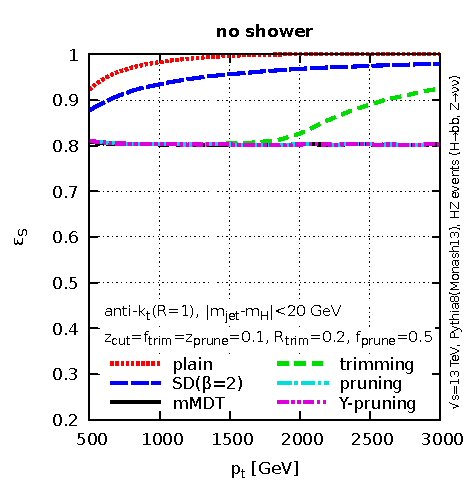
\includegraphics[width=0.48\textwidth,page=1]{figures/groomed-signal-eff.pdf}}%
  \hfill%
  \subfloat[]{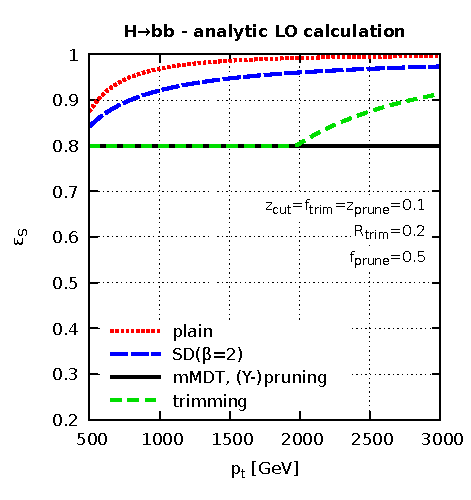
\includegraphics[width=0.48\textwidth,page=1]{figures/groomed-signal-analytic.pdf}}
  %
  \caption{Higgs reconstruction efficiency as obtained from Pythia8
    (left) and a LO analytic calculation (right). The Pythia8
    simulation is done at parton level with both the initial-state and
    final-state shower switched off. Different curves correspond to
    different taggers (see \eg
    Fig.~\ref{fig:groomers-pythia-v-analytic} for
    details).}\label{fig:groomers-pythia-sig-hard}
\end{figure}

We can compare these results to Monte Carlo simulations. 
%
For simplicity, we use the Pythia8 generator, simulating the
associated production of a Higgs and a Z boson, where the latter decays into (invisible)
neutrinos and the Higgs boson decays to a $b\bar b$ pair. We
reconstruct the jets using the anti-$k_t$ algorithm with $R=1$ and
select the hardest jet in the event, imposing a cut on the jet
$p_t$. The jet is then tagged/groomed and we deem the
jet as tagged if the jet mass after grooming is within
$\delta M=20$~GeV of the Higgs mass, \ie between 105 and 145~GeV,
with $m_H=125$~GeV.
%
We study the Higgs tagging efficiency as a function of the $p_t$ cut
applied to the initial jet.

To compare to the analytic results, Eq.~\eqref{eq:lo-grm-sig-eff}, we
simulate parton-level results switching off both the initial and
final-state showers.
%
Results are presented in Fig.~\ref{fig:groomers-pythia-sig-hard}
(left) together with our simple analytic results (right).
%
The analytic results capture very well the behaviour
observed in the Monte Carlo simulations. In particular, all the
features discussed above can be observed: the mMDT and (Y-)pruning
remain constant as a function of the jet $p_t$ and the efficiency of
the other taggers/groomers increases with $p_t$, with the plain jet
efficiency increasing more rapidly than the \SD one.
%
With our choices of parameters, the transition $\rho=\zcut$ (or
$\ftrim$) corresponds to a $p_t\approx 400$~GeV and is thus not
visible on the plot.
%
For trimming one sees the transition between the region dominated by
the $z>\ftrim$ condition at lower $p_t$ and the region dominated by
the $\theta<\rtrim$ condition at larger $p_t$. The transition between
the two regions happens at
$p_t=m_H/(R_\text{trim}\sqrt{\ftrim})\approx 2$~TeV, in agreement with
what is observed on the plot.


\begin{figure}[t!]
  \subfloat[]{\includegraphics[width=0.48\textwidth,page=2]{figures/groomed-signal-eff.pdf}}%
  \hfill%
  \subfloat[]{\includegraphics[width=0.48\textwidth,page=6]{figures/groomed-signal-eff.pdf}}
  %
  \caption{Higgs reconstruction efficiency as obtained from
    Pythia8. The simulation is done at parton level, including only
    final-state radiation. The right plot shows the effects of
    final-state shower, \ie the ratio to the efficiencies obtained
    with no final-state shower. See
    Fig.~\ref{fig:groomers-pythia-sig-hard} for other
    details.}\label{fig:groomers-pythia-sig-fsr}
\end{figure}


\paragraph{Final-state radiation.}
%
We now move to consider the effects of final-state radiation (FSR) on
signal efficiency. The final-state gluons radiated by the $q\bar q$
pair can be groomed away, resulting in a
decrease of the reconstructed jet mass. The jet mass can therefore fall
below our lower cut $m_H-\delta M$ on the mass meaning that FSR is
expected to reduce the signal efficiency.
%
We know from our discussion of QCD jets in the previous sections that
the emissions in a final-state shower can have
logarithmically-enhanced effects on jet substructure observable. From
an analytic viewpoint, these emissions would then have to be resummed
to all orders.

While in practice it would be insightful to first consider the
${\cal {O}}(\alpha_s)$ case where a single gluon is emitted by the
$q\bar q$ pair --- similarly to what was done for the one-gluon
emission case for QCD jets at LO ---, we directly turn to the
situation where we include the full parton shower. We first discuss
the case of final-state radiation --- by the $q\bar q$ pair --- and
discuss initial-state radiation below.
%
We therefore run Pythia8 simulations, still at parton level, but this
time including final-state shower (and with the initial-state shower
still disabled).
%
The resulting efficiencies are plotted in
Fig.~\ref{fig:groomers-pythia-sig-fsr}.
%
If one focuses on the right-hand plot, showing the ratio of the
efficiencies obtained with final-state radiation to the efficiencies
obtained without, we see a relatively small effect of FSR for all the
substructure algorithms, even very small for the plain jet and \SD. This is not true for
trimming, for which the effect of FSR is to a large extend constant in $p_t$.
%
In the case of trimming, we see that at small $p_t$, more precisely
for $p_t<m_H/(R_\text{trim}\sqrt{\zcut})\approx 2$~TeV, \ie
$\rho>\zcut\rtrim^2$, the effect of FSR increases when
decreasing $p_t$.

From an analytic perspective, the emission of FSR gluons can come with
an enhancement proportional to $\log(\delta M^2/M_H^2)$ for a
small-width mass window, or a logarithm of $\zcut$, $\ftrim$ or
$\zprune$, all associated with soft gluon emissions. This is what
drives the $p_t$ independent loss of signal efficiency in the case of
mMDT and (Y-)pruning in Fig.~\ref{fig:groomers-pythia-sig-fsr}. For
the plain jet and \SD, this effect becomes suppressed by a power of
$M_H/p_t$.
%
Furthermore, in the case of trimming, due to the fixed trimming
radius, the effect of final-state radiation is also enhanced by
collinear logarithms of $\rho/\rtrim^2$ for $\rtrim^2\ll\rho\ll 1$,
\ie in the intermediate $p_t$ region. This logarithmically-enhanced
effect is the main reason for the slow rise of the trimming signal
efficiency between 500~GeV and 2~TeV.


\begin{figure}[t!]
  \subfloat[]{\includegraphics[width=0.48\textwidth,page=3]{figures/groomed-signal-eff.pdf}}%
  \hfill%
  \subfloat[]{\includegraphics[width=0.48\textwidth,page=7]{figures/groomed-signal-eff.pdf}}
  %
  \caption{Left: Higgs reconstruction efficiency obtained with Pythia8
    at parton level. Right: effects of initial-state radiation, \ie
    ratio to the efficiencies obtained with only final-state
    shower. See Fig.~\ref{fig:groomers-pythia-sig-hard} for other
    details.}\label{fig:groomers-pythia-sig-isr}
\end{figure}

\paragraph{Initial-state radiation.}
%
Next, we discuss the effect of initial-state radiation
(ISR). Compared to the case of FSR, capturing an ISR gluon in the
(groomed) jet shifts its mass up, meaning that it can go above
$M_H+\delta M$, again lowering the efficiency.
%
This effect is again potentially enhanced by a logarithm of
$\delta M^2$.
%
The results of our Monte Carlo study of ISR effects is presented in
Fig.~\ref{fig:groomers-pythia-sig-isr}, where we a small effect for
mMDT, SoftDrop, trimming and pruning, a slightly larger effect for
Y-pruning and a sizeable loss of efficiency in the case of the plain
jet.

In the case of the plain jet mass, one does get an enhancement of ISR
effects by a logarithm of $M_H\,\delta M/p_t^2$, responsible for the
loss of signal efficiency when increasing $p_t$.
%
For groomed jets, one can show (see~\cite{Dasgupta:2015yua}) that this
logarithm is typically suppressed by a power of $M_H/p_t$ (related to
the fact that the groomed jet radius decreases with $p_t$) and is
replaced by a less harmful logarithm of $\zcut$, $\ftrim$ or $\zprune$
coming from situations where a large-angle ISR gluon passes the
grooming condition.
%
The case of Y-pruning is a bit more complex as even when an ISR
emission fails the pruning condition, it could have still affected
(increased) the pruning radius and cause the Y-pruning condition to
fail.  This is the main source of the decrease of the signal
efficiency observed for Y-pruning at large $p_t$ in
Fig.~\ref{fig:groomers-pythia-sig-isr}.


\begin{figure}
  \subfloat[]{\includegraphics[width=0.48\textwidth,page=4]{figures/groomed-signal-eff.pdf}}%
  \hfill%
  \subfloat[]{\includegraphics[width=0.48\textwidth,page=8]{figures/groomed-signal-eff.pdf}}
  %
  \caption{Left: Higgs reconstruction efficiency obtained from
    Pythia8 at hadron level. Right: hadronisation effects, \ie ratio
    to parton-level efficiencies. See
    Fig.~\ref{fig:groomers-pythia-sig-hard} for
    details.}\label{fig:groomers-pythia-sig-hadr}
\end{figure}


\begin{figure}
  \subfloat[]{\includegraphics[width=0.48\textwidth,page=5]{figures/groomed-signal-eff.pdf}}%
  \hfill%
  \subfloat[]{\includegraphics[width=0.48\textwidth,page=9]{figures/groomed-signal-eff.pdf}}
  %
  \caption{Left: Higgs tagging efficiency obtained from a full
    Pythia8 simulation. Right: UE effects, \ie ratio to
    efficiencies with UE switched off. See
    Fig.~\ref{fig:groomers-pythia-sig-hard} for
    details.}\label{fig:groomers-pythia-sig-ue}
\end{figure}

\paragraph{Non-perturbative effects.} The effects of hadronisation and
of the UE are presented in
Figs.~\ref{fig:groomers-pythia-sig-hadr}
and~\ref{fig:groomers-pythia-sig-ue}, respectively.
%
Hadronisation corrections are generally small, especially for groomed
jets where they are almost negligible. In the case of the plain jet,
hadronisation effects tend to increase at large $p_t$ but the
correction remains within 10\%.
%
The case of UE corrections is more striking: the signal
efficiency in the case of the plain jet is severely affected by
UE contamination.
%
After grooming, the UE correction becomes very small
across the whole range of $p_t$ studied. This is directly related to
the initial idea behind grooming, namely to reduce soft contamination
--- and hence UE effects --- by removing soft and
large-angle emissions in the jet.

Once all effects are taken into account, the efficiency for groomed
jets is found to be close to the initial prediction at leading order,
with small corrections from ISR, FSR and non-perturbative
effects. Trimming has a small extra $p_t$ dependence at intermediate
$p_t$ coming from final-state radiation, and Y-pruning has a small
loss of signal efficiency at large $p_t$ due to initial-state
radiation.
%
This picture is contrasted by what happens in the case of the plain
jet where ISR and, in particular, the UE have a sizeable
effect, and hadronisation corrections are larger than for groomed
jets.
%
A consequence of this resilience of groomed jets is that, despite the
smaller signal efficiency at leading-order,
cf.~Fig.~\ref{fig:groomers-pythia-sig-hard}, the groomed jet signal
efficiency is clearly larger than the ungroomed signal efficiency once
all effects beyond LO are included.


%% GS helper for auctex
%%% Local Variables:
%%% mode: latex
%%% TeX-master: "notes"
%%% End:

%  LocalWords:  Eq eq NNLL parton's Eqs UE Monash NLL expectably FSR
%  LocalWords:  ISR
